Until now, we have seen how to achieve secure communication  over an insecure channel, but not discussed yet how keys are shared and managed. Indeed these are some of the main problems of symmetric schemes, especially in an open system like the Internet. For a group of $n$ entities where everyone wants to communicate with each other, the total number of secret keys that need to be generated is $\binom{n}{2} \approx \mathsf{O}(n^2)$, and these need to be distributed over a secure channel that is not always present.
Even if partial solutions were built to overcome these problems, they were not enough.
The first step to fully solve these problems was made in 1976 by Whitfield Diffie and Martin Hellman in a paper called "New Directions in Cryptography". With this paper, they laid the foundation for asymmetric schemes. These schemes use two different keys called the \emph{public} and \emph{private} key. The first one is used to encrypt the message, while the second one to decrypt the ciphertext.\\
So, a public key scheme is a tuple $(\mathsf{Gen}, \mathsf{Enc}, \mathsf{Dec})$ such that:
\begin{itemize}
    \item{$\mathsf{Gen}(\cdot)$: takes as input the security parameter $n$ and outputs a pair of key $(pk, sk)$, which are the public and the secret (private) key, respectively.}
    \item{$\mathsf{Enc}(\cdot)$: takes as input a public key $pk$ and a message $m$ to output the ciphertext $c \leftarrow \mathsf{Enc}_{pk}(m)$.}
    \item{$\mathsf{Dec}(\cdot)$: takes as input a secret key $sk$ and a ciphertext $c$ to output the message $m := \mathsf{Dec}_{sk}(c)$.}
\end{itemize}
It's also required that for every $n$, every possible pair $(pk, sk)$, and every $m$ it holds that
$$
m = \mathsf{Dec}_{sk}(\mathsf{Enc}_{pk}(m))
$$
To establish a communication between two entities Alice and Bob, first the key pairs $(A_{pk}, A_{sk})$ and $(B_{pk}, B_{sk})$ are generated, then both public keys are shared among the entities and used to encrypt messages. Imagine that Alice wants to send a message $m$ to Bob, Alice crafts the ciphertext using Bob's public key $c \leftarrow  \mathsf{Enc}_{B_{pk}}(m)$, then sends it to Bob that will decode the message with his secret key $m = \mathsf{Dec}_{B_{sk}}(c)$.\\
In the scenario where $n$ entities participate in the communication, the number of keys involved is $2n$ and every public key can be freely distributed through insecure channels.
\begin{figure}[H]
    \centering
    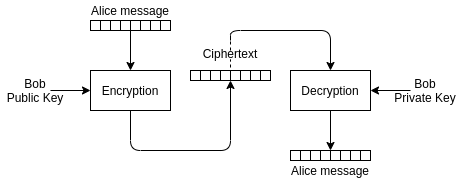
\includegraphics[width=0.6\textwidth]{img/public-key/encryption.png}
    \caption[Public key encryption example.]{Public key encryption example. Alice uses Bob's public key to encrypt the messages she wants to send.}
\end{figure}
